\documentclass[12pt]{article}

\usepackage{notestyle}

\graphicspath{{./img/}}


\title{Note Web Application}
\author{Brendon Mendicino}



\begin{document}

\maketitle
\newpage
\tableofcontents
\newpage



\section{ Introduction}
JS is backward compatible, to be able to use the previous features is use the directive:
\begin{lstlisting}[language=js]
"use strict";
\end{lstlisting}
JS has primitive types and non-primitive types, JS is also and strongly typed language, the primitive types are: string, number, boolean, null, undefined. The non-primitive are the objects, which can be: array, function, user-defined.

The all possible false values in JS: \verb|0, -0, NaN, undefined, null, ''|, in JS there are two main comparison operators:
\begin{lstlisting}[language=js]
a == b    // equal, convert types and compare
a === b   // strict equal, inhibits automatic type conversion
\end{lstlisting}
In JS you can create variable with:
\begin{lstlisting}[language=js]
// modern
let a = 10;    // can be changed
const b = 'a'; // constant

// old
var k = 9;
j = 30;
\end{lstlisting}
The difference between null and undefined, is that variable with null they old a value which is null, on the other way if a variable is declared and nothing is associated with it the value olds by default undefined.

A scope is defined by a \textbf{block}, which is created with \texttt{{ ... }}

There two kinds of \texttt{foreach} in JS, using \texttt{in} allows iterating over objects, while \texttt{of} allows iterating over iterable objects:
\begin{lstlisting}[language=js]
for (let a in object) {
  ...
}

for (let b of iterable) {
  ...
}
\end{lstlisting}
Using arrays:
\begin{lstlisting}[language=js]
let a = [1, 2, 'ok', false];
let b = Array.of(1, 2, true);
a.push(5);      // append an element
b.unshift(2);   // insert at the beginning

let copy = Array.from(a);  // shallow copy, it does not deep copy
\end{lstlisting}
The \textbf{destructuring assignment} can be done, it extracts the values from the mast left-hand side:
\begin{lstlisting}[language=js]
let [x, y] = [1, 2];
[x, y] = [y, x]     // swap
\end{lstlisting}
The \textbf{spread operator} (\texttt{...}) expands on iterable object into it's values:
\begin{lstlisting}[language=js]
let [x, ...y] = [1, 2, 3, 4];      // y == [2, 3, 4]

const a = [1, 2];
const b = [0, ...a, 3]; // [0, 1, 2, 3]
\end{lstlisting}
Spreading can be from the left or from the right, usually the spread operator is used for copying array:
\begin{lstlisting}[language=js]
const a = [1, 2];
const b = [...a];
\end{lstlisting}
A \textbf{string} is JS is an immutable type (like python) encoded in Unicode. The \textbf{template literals} can be done with the \textbf{tick} operator \texttt{``} (expression like Kotlin):
\begin{lstlisting}[language=js]
let name = 'Bre';
let sur = 'Mend';
// Template literal
let fullName = `${name} ${sur}`;
\end{lstlisting}


\subsection{Objects}
JS is \textbf{prototype based language}, which means that there are no declarations of classes. In JS property names must be strings and can be modified, the value of the property can be any other type of type or object. To create and object in JS you use curly braces and the defined properties:
\begin{lstlisting}[language=js]
const movie = {
  title: 'Inception',
  genre: 'sci-fi',
  duration: 180
}

console.log(movie)
console.log(movie['title'])
console.log(movie.title)
\end{lstlisting}
It is also possible to add a property by simple assigning a new name to a type, it is also possible to delete a property with the keyword \texttt{delete}. There are two helper functions:
\begin{itemize}
  \item \texttt{Object.key(object)}: return only the key;
  \item \texttt{Object.entries(object)}: return an array with the key and value;
\end{itemize}
To copy an object it is possible to use:
\begin{lstlisting}[language=js]
const copied = Object.assign({}, original)
const withSpread = {...original}    // it also possbible to use the spread operator

// assign can also be used to merge objects
const merged = Object.assign({}, copied, {something: 'test'})
\end{lstlisting}


\subsection{Functions}
In JS functions are objects, so it is possible to assign a function to a property or use it in a parameter in another function. There three possible ways to define a function:
\begin{lstlisting}[language=js]
// 1. Function
function do(a, b = 1) {
  ...
}

// parameters can also hava a deafult value
function some(par1, par2, ...variable) { // ... is the 'rest' operator, like varargs, rest parameters can be iterated
  ...
}

// 2. Function Expression
const fn = function(params) { }

// 3. Arrow Function
const func = (params) => { }
\end{lstlisting}
In JS \textbf{Closure} can be created, with closure it is possible to use parameters of the scope where the function is defined, even if that scope does not exist any more.
\begin{lstlisting}[language=js]
function greeter(name) {
  const myname = name;

  const hello = () => {
    return "Hello " + myname;
  }

  return hello;
}

const helloTest = greeter('test');

console.log(helloTest());   // 'Hello test'
\end{lstlisting}
To create an object there are also \textbf{constructor functions}:
\begin{lstlisting}[language=js]
function Movie(title, director, duration) {
  this.title = title;
  this.director = director;
  this.duration = duration;
  this.isLong = () => this.duration > 120;
}

cosnt movie = new Movie('Inception', 'Nolan', 180);
console.log(movie.isLong);  // true
\end{lstlisting}


\subsection{Dates}
We use \texttt{dayjs()} objects in JS to build a data, it is an external library. The return of \texttt{dayjs()} fetches the time from the locale time, other than that it can create a data from ISO8601 strings, 8 digit dates, etc. To install this library: \texttt{\$ npm install dayjs}. The string value of the standard format is in ISO9601 in UTC time, it's important to remember that the days and the month inside the object start \emph{counting from 0}. Other than that the library has some methods to compare different \texttt{dayjs} objects, also by choosing the level of \emph{granularity} (year, month, day, ...).
\begin{lstlisting}[language=js]
const date = dayjs('2023-03-15');
const now = dayjs();

now.isAfter(date, 'day');  // comparing 'now' and 'date' by day
\end{lstlisting}


\subsection{Asynchronous Programming}
In JS when passing functions to other functions it's called a \textbf{callback}, this functions can be \emph{synchronous} or \emph{asynchronous}.
\begin{lstlisting}[language=js]
function logQuote(quote) {
  console.log(quote);
}

funtion createQuoute(quote, callback) {
  const myQuote = `Like I always say, ${quote}`;
  callback(quote);
}

createQuote('sium', logQuote);
\end{lstlisting}
In order to have functional features in language there some need properties:
\begin{itemize}
  \item \emph{functions as first class citizen};
  \item \emph{higher-order functions};
  \item \emph{function composition};
  \item \emph{call chaining};
\end{itemize}
In JS arrays have functional methods, for example:
\begin{lstlisting}[language=js]
a.forEach(item => ...);   // action on every element of the array
a.every(x => x > 10);     // return true if all elements satisfy the condition, false otherwise
a.some(x => x < 10);      // return true if at least one element satisfy the condition
a.map(x => `${x}`);       // return a new array with every element mapped to a new one
a.filter(x => x === 0);   // return a new array with all elements that satisfy the condition
a.reduce((x, y) => x + y, 0);   // return a reduced value
\end{lstlisting}
Even though JS is executed on a single thread it is possible to create concurrent code, for example a function that allows to excute a callback after a certain amount of time is the \texttt{setTimeout()} function:
\begin{lstlisting}[language=js]
const f = (task) => {
  // do something
};

setTimeout(f, 2000, task);
\end{lstlisting}
This is possible because JS runs in the \textbf{Event Loop}, which periodically checks if there are some part of the code that needs to be executed.

There is a function that allows asynchronous callback after a timeout:
\begin{lstlisting}[language=js]
const onesec = setTimeOut(() \implies {
  console.log('1 second has passed');
}, 1000);
\end{lstlisting}
There is also the \texttt{setInterval()} function that periodically runs:
\begin{lstlisting}[language=js]
const period = setInterval(() => {}, 2000);
clearInterval(period);
\end{lstlisting}


\subsubsection{Database Access (SQLite)}
The module for \texttt{sqlite3} allows calling sql queries via his APIs, first there needs to be an open with the database, to open a connection use:
\begin{lstlisting}[language=js]
const sqlite = require('sqlite3');

const db = new sqlite.Database('exams.sqlite', 
  (err) => { if (err) throw err; });
\end{lstlisting}
Example of query:
\begin{lstlisting}[language=js]
let result = [];
let sql = "SELECT * FROM course LEFT JOIN score ON course.code=score.coursecode";
db.all(sql, (err, row) => {
  if (err) throw err;
  for (let row of rows
});
\end{lstlisting}
The problem with execution this queries is that they are \emph{all asynchronous}, and they can cause race conditions. The solution to this problem are \texttt{Promise}, which helps simplyfing asynchronous programming. A \texttt{Promise} handles a \texttt{resolve} and a \texttt{reject} which needs to be called when the callback fails or succedes. The values passed to \texttt{resolve} can be accessed by in the \texttt{then} method, which gets called when the \texttt{Promise} is completed.
\begin{lstlisting}[language=js]
function waitPromise(duration) {
  return new Promise((resolve, reject) => {
    if (duration < 0) {
      reject(new Error('...'));
    } else {
      setTimeout(resolve, duration);
    }
  }
}

waitPromise(1000).then((result) => {
  colsole.log('Success :', result);
}).catch((error) => {
  colsole.log('Error :', error);
});
\end{lstlisting}
A promise has 3 main methods: \texttt{then}, \texttt{catch}, \texttt{finally}, which are similar behaviour to the try catch block in Java. Promises can also work concurrently with \texttt{Promise.all()} or \texttt{Promise.race()}.

\subsubsection{Await/Async}
The keywords \texttt{async} and \texttt{await} allows to convert pieces of code to a \texttt{Promise}:
\begin{lstlisting}[language=js]
function resolveAfter2Seconds() {
  return new Promise(resolve => {
    setTimeout(() => {
      resolve('resolved');
    }, 2000);
  });
}

async function asyncCall() {
  console.log('calling');
  const result = await resolveAfter2Seconds();
  console.log(result);
}

asyncCall();  // this returns is a promise
\end{lstlisting}
In fact a function marked as \texttt{async} returns a promise.

\hfill

This method can be combined with the database queries:
\begin{lstlisting}[language=js]
async function main() {
}

main();
\end{lstlisting}




\newpage
\section{HTML/CSS}

CSS has different mesuraments units:
\begin{itemize}
  \item \texttt{em}: unit size relative to the font size present in the current element;
  \item \texttt{rem}: unit relative to the font size of the root element;
  \item \texttt{vw}: relative to $1\%$ of the width of the viewport;
  \item \texttt{vh}: relative to $1\%$ of the height of the viewport;
\end{itemize}
CSS has aldo \textbf{pseudo selector} which represent changes based on the state of an element.
\begin{lstlisting}[language=html]
a:visited { color: green; }
\end{lstlisting}
In CSS there 4 position schemes: \textbf{static}, \textbf{relative}, \textbf{absolute}, \textbf{fixe}.

In CSS the flex schema allows for direct control over the element of the page, it allows modifying: direction, sizes, alignment, position, spacing, ...

In CSS the \texttt{\~} selector is called \textbf{subsequent sibling combinator}, the element represented by the first sequence precedes (not necessarily immediately) the element presented by the second one.
\begin{figure}[H]
  \centering
  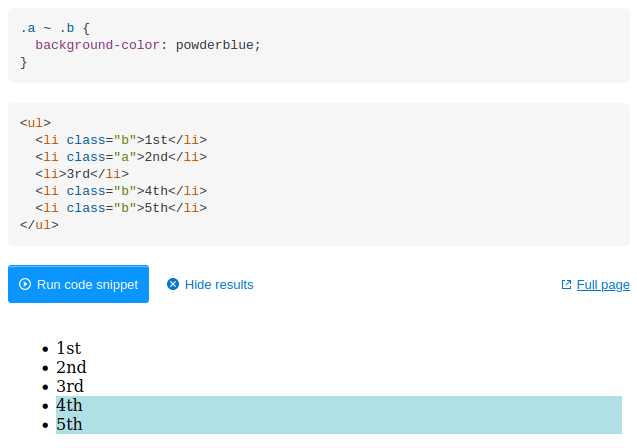
\includegraphics[width=0.8\textwidth]{subsequent-sibling-operator.png}
  \caption{Subsequent Sibling Operator}
  \label{fig:subsequent-sibling-operator}
\end{figure}

\subsection{Responsive}
It's possible to achieve a responsive layout by using \texttt{media query}:
\begin{lstlisting}[language=html]
@media(min-width:900) { }
\end{lstlisting}


\section{JS inside HTML}
The perferred way to include javascript code inside the html is:
\begin{lstlisting}[language=js]
<script async src="script.js"></script>
// or better
<script defer src="script.js"></script>
\end{lstlisting}
Where does the code run?


The main objects of the browser:
\begin{itemize}
  \item \textbf{DOM}: Document Object Model 
  \item \textbf{BOM}: Browser Object Model, non-standard
\end{itemize}
The BOM has a \texttt{window} object, which contains: \texttt{console, document, history, location, localStorage, sessionStorage}.

The DOM is 

The DOM can be accessed like a squence of Nodes. To find a node there are vaarius methods, like:
\begin{itemize}
  \item \texttt{document.getElementById(value)}
  \item \texttt{document.getElementsByTagName(value)}
  \item \texttt{document.getElementsByClassName(value)}
  \item \texttt{document.querySelector(css)}
  \item \texttt{document.querySelectorAll(css)}
\end{itemize}
From each node there are many mothod to access all the neigbhor nodes.




\subsection{Event Handling}
...




\newpage
\section{React}
React is a framework that allows DOM manipulation with a level of abstractions, and while using it won't be necessary to touch the DOM directly.

React has a functional approach, which allows bulding a web page in a declarative approach. On any change that is acted on a component all the other components are rerendered. Fot this reason React has a \textbf{virtual DOM} which is built on top of the DOM which will eventually push his changes to the original DOM.

The basic information that are shared between components are the \texttt{state} and \texttt{props} (properties), which are passed to functions inside the component.

On re-rendering when the virtual DOM is stabilized, the difference between the virtual DOM and the DOM are computed and only then the changes are moved on the actual DOM, this is why this re-rendering is not so heavy.

There are event that are normalized across the browser, this are called \textbf{synthetic events}.

If we want to write a minimal React application:
\begin{lstlisting}[language=js]
const container = document.getElementById('root');

const root = createRoot(container);
root.render(<h1>Hello, world!</h1>);
\end{lstlisting}
React uses \texttt{jsx} that are translated into \emph{react elements}, this \texttt{jsx} will be then be translated to plain javascript by React. To define a component in React we do:
\begin{lstlisting}[language=js]
const BlogPostExcerpt = (props) => {
  return (
    <div>
      <h1>Title</h1>
      <p>{props.content}</p>
    </div>
  )
}
\end{lstlisting}
There are two types of component: 
\begin{itemize}
  \item \textbf{presentation component} don't manage the state;
  \item \textbf{container component} manages the state of all his children;
\end{itemize}
\texttt{props} can only be passed from a parent to his children, if the changes shoul be performed from the a children to a parent then, a callback needs to be passed.
\begin{center}
  \boxed{\text{React flow: view $\implies$ actions $ \implies $ state $ \implies $ view $ \implies \dots $}}
\end{center}
\begin{itemize}
  \item A \textbf{state} is always \textbf{owned be one compoment}.
  \item Changing state on a childred should not affect the state of a parent.
\end{itemize}
To create a React application
\begin{lstlisting}[language=]
$ npm create vite@latest my-app
// Choose React, javascript + SWC
$ cd my-app
$ npm install
$ npm run dev
\end{lstlisting}
In \texttt{jsx} the attributes of a component (\texttt{props}) are translated into js objects
\begin{lstlisting}[language=js]
color="red" -> {color: "red"}
tone={2} -> {tone: 2}
// it's possible compute exressions
color={active ? 'green' : 'red'}
\end{lstlisting}
Some attributes in HTML do not a value like \texttt{selected} \texttt{disabled}, but in \texttt{jsx} they can have a value: \verb|selected={true}|

In React when using a list it's mandatory to use give a key to each element of the list (the key is unique in the list, not globally), this is done because React internally can recognise if the list has changed, if this is not done there are undefined behaviur in the page.
\begin{lstlisting}[language=js]
<li key={todo.id}>{todo.text}</li>
\end{lstlisting}
When returning a gruop of components they should always be packed in a root component, when returing a  group of components there is \emph{React Fragment} which makes it more easy.

















\end{document}

%% vim: ts=2 sts=2 sw=2 et
